\chapter{Entorno de desarrollo \textit{MIPS32}}\label{ch:entorno-de-desarrollo-mips32}

El desarrollo de \textit{JAMS} está dividido en dos secciones:
la aplicación base y el entorno de desarrollo \textit{MIPS32}.
\textit{JAMS} da soporte al lenguaje ensamblador \textit{MIPS32}
creando una \textbf{capa sobre la aplicación base},
aprovechando todas las herramientas y características explicadas anteriormente.
En este capítulo se abordarán las capacidades de este entorno,
documentando el ensamblador, el simulador y el editor junto
con sus componentes esenciales.


\section{Ensamblador \textit{MIPS32}}\label{sec:ensamblador-mips32}

El ensamblador \textit{MIP32} de \textit{JAMS} es un ensamblador avanzado
usado para ensamblar proyectos \textit{MIPS32}.
Este ensamblador soporta características avanzadas empleadas
comúnmente al programar en ensamblador, como las macros,
las etiquetas globales o las referencias relativas.

\noindent El ensamblador ensambla el código de un proyecto en cuatro pasos:
descubrimiento, expansión, asignación de direcciones y asignación de valores.
Se utilizará el siguiente programa para comentar los
diferentes pasos del ensamblador:

\begin{lstlisting}[frame=single,label={lst:example.asm}]
    .macro print ( %string )
    .data
text:   .asciiz %string
    .text
    la $a0, text
    li $v0, 4
    syscall
    .endmacro

    .macro printJams ()
    print ("Welcome to JAMS!\n")
    .endmacro

    .text
    .globl main print
main:
local:
    printJams ()
\end{lstlisting}

\subsection{Descubrimiento}\label{subsec:descubrimiento}

En este paso el texto del proyecto se \textbf{descompone en sus primitivas},
permitiendo al ensamblador entender los diferentes componentes de cada línea.
Al final de este paso, las etiquetas globales y las etiquetas de archivo
(etiquetas no definidas dentro de una macro) \textbf{son registradas sin
ningún valor asignado}.

\noindent Las macros de cada archivo también son registradas.
El identificador de una macro es definido por su nombre concatenado
al número de parámetros que necesitan.
Este procedimiento se realiza para dar soporte a la sobrecarga de macros.
En el caso de la macro $print$, su identificador sería $print-1$.

\begin{lstlisting}[frame=single,label={lst:descubrimiento}]
Etiquetas globales:
main - XXXXXXXX

Etiquetas del archivo:
local - XXXXXXXX

Macros globales:
print-1

Macros del archivo:
printJams-0
\end{lstlisting}

\subsection{Expansión}\label{subsec:expansion}

En este paso, las llamadas a macros son invocadas,
insertando el código de la macro en la posición de la llamada.
Este código efectúa el primer paso del ensamblador mientras es añadido.
Al ser insertado justo después de la llamada, el código de la macro
también será expandido.

\begin{lstlisting}[frame=single,label={lst:expansion}]
main:
local:
    # Macro printJams-0
    # Macro print-1
    .data # Data returns the previous address.
text:   .asciiz "Welcome to JAMS!\n"
    .text
    la $s0, text
    li $v0, 4
    syscall
    # Endmacro print-1
    # Endmacro printJams-0
\end{lstlisting}

\subsubsection{Alcance}\label{subsubsec:alcance}

Las etiquetas y macros que están dentro de una macro
\textbf{tienen un alcance diferente al del archivo}.
Si la macro es global, el alcance es considerado hijo del alcance global
y no podrá acceder a las etiquetas del archivo que lo invoca.
Si la macro es local, el alcance es considerado hijo del alcance del archivo.

\noindent Cuando un alcance es hijo de otro alcance,
\textbf{el hijo podrá acceder a las etiquetas y macros de su padre}.
El hijo también podrá definir nuevas etiquetas y macros con el mismo
identificador que una etiqueta o macro de su padre.
Aunque este comportamiento está permitido, \textbf{el hijo solo podrá acceder
al elemento que él define}.
Esta funcionalidad es llamada \textbf{ocultamiento o \textit{shadowing}}.

\subsection{Assignación de direcciones}\label{subsec:assignacion-de-direcciones}

Una vez el ensamblador haya expandido las macros,
se asignan las direcciones de todas las instrucciones,
etiquetas y directivas que requieran dirección.
Estas direcciones se asignan de manera secuencial.
Existen directivas que pueden modificar el flujo de la asignación,
como es el caso de la directiva $.text$.

\begin{lstlisting}[frame=single,label={lst:address-assignation}]
main:
local:
                    # Macro printJams-0
                    # Macro print-1

0x00400000          .data # Data returns the previous address.
0x10010000      text:    .asciiz "Welcome to JAMS!\n"
0x10010010          .text

                    # la is a pseudo-instruction and
                    # it will be split in two instructions
0x00400000          la $s0, text
0x00400008          li $v0, 4
0x0040000c          syscall

                    # Endmacro print-1
                    # Endmacro printJams-0
\end{lstlisting}

\subsection{Asignación de valores}\label{subsec:asignacion-de-valores}

Como paso final, el ensamblador insertará en memoria los valores
que representan las directivas e instrucciones.

\begin{lstlisting}[frame=single,label={lst:value-assignation}]
                    # Macro printJams-0
                    # Macro print-1

0x10010000          Welcome to JAMS!\n\0
0x00400000          0x3c011001 # la $a0, text
0x00400004          0x34240000
0x00400008          0x24020004 # li $v0, 4
0x0040000c          0x0000000c # syscall

                    # Endmacro print-1
                    # Endmacro printJams-0
\end{lstlisting}

\subsection{Características avanzadas}\label{subsec:características-avanzadas}

El ensamblador permite el uso de técnicas avanzadas en
el desarrollo de aplicaciones en lenguaje ensamblador.

\subsubsection{Referencias relativas}\label{subsubsec:referencias-relativas}

Una directiva o instrucción puede \textbf{referenciar a una etiqueta de manera
relativa} con las referencias especiales $+$ y $-$.
La referencia $+$ hace referencia a la etiqueta siguiente.
La referencia $-$ hace referencia a la etiqueta anterior.
Las referencias relativas \textbf{solo pueden hacer referencia
a etiquetas del mismo alcance}.
No pueden hacer referencia a etiquetas de un alcance mayor.

\begin{lstlisting}[frame=single,label={lst:relative-reference}]
main:
    li $s0, 0
    li $s1, 10
loop:
    printJams ()
    addi $s0, $s0, 1
    bne $s0, $s1, -
\end{lstlisting}

\subsubsection{Macros anidadas}\label{subsubsec:macros-anidadas}

Una macro puede ser definida dentro de otra macro.
Esto es conocido como una \textbf{macro anidada}.
Esta macro solo podrá ser accedida en el alcance de la macro
en la que está declarada.

\begin{lstlisting}[frame=single,label={lst:nested-macro}]
    .macro printJams ()
    .macro print (%string)
    .data
text:   .asciiz %string
    .text
    la $a0, text
    li $v0, 4
    syscall

    .endmacro
    print ("Welcome to JAMS!\n")
    .endmacro
\end{lstlisting}


\section{Instrucciones}\label{sec:instrucciones}

Las instrucciones son la parte más importante de un lenguaje ensamblador.
JAMS permite crear y gestionar instrucciones de una manera modular.

\subsection{Estructura de una instrucción}\label{subsec:estructura-de-una-instruccion}

Todas las instrucciones implementan la interfaz \textbf{Instruction}.
Esta interfaz define conceptos básicos de una instrucción,
como su nombre, su mnemónico, su documentación o sus parámetros.
Esta interfaz también define los métodos $match$,
usada para comprobar si un mnemónico y un conjunto de parámetros
representan una instrucción.
Estos métodos son utilizados por el ensamblador y el editor para saber qué
instrucción define una línea.
Por último, la interfaz define el método \textit{assemble}, el
cual traduce la instrucción en un conjunto de instrucciones ensambladas.
Este método debe ser implementado por las clases hijas.
Esta interfaz es implementada por dos clases abstractas básicas:
$BasicInstruction$ y $PseudoInstruction$.

\subsection{Instrucciones básicas}\label{subsec:instrucciones-basicas}

Las instrucciones básicas (representadas por la clase abstracta
$BasicInstruction$) representan instrucciones normales del ensamblador.
Estas instrucciones tienen una traducción directa a código máquina.
Esta clase abstracta define elementos más concretos, como el código de operación,
la unidad aritmético-lógica donde la instrucción debe ejecutarse y
un nuevo método $match$ que permite saber si un código de instrucción
representa la instrucción.
Esta clase define los métodos abstractos $assembleBasic$
y $assembleFromCode$.
Estos métodos permiten crear un elemento de tipo $AssembledInstruction$
mediante un código de instrucción o un conjunto de parámetros.
El método $assemble$ de la interfaz $Instruction$
está implementada por esta clase.

\noindent Todas las instrucciones básicas requieren dos
constantes globales en su implementación:
\begin{itemize}
    \item \textbf{MNEMONIC:} es un $String$ que define
    el mnemónico de la instrucción.
    \item \textbf{PARAMETER\_TYPES:} es un elemento de tipo
    $InstructionParameterTypes$ que representa
    los tipos de los parámetros de la instrucción.
\end{itemize}

\begin{lstlisting}[language=Java,style=java,frame=single,label={lst:basic-instruction}]
public class InstructionAbsDouble extends
    BasicRFPUInstruction<InstructionAbsDouble.Assembled> {

    public static final String MNEMONIC = "abs.d";
    public static final InstructionParameterTypes PARAMETER_TYPES =
        new InstructionParameterTypes(
            ParameterType.EVEN_FLOAT_REGISTER,
            ParameterType.EVEN_FLOAT_REGISTER
        );
}
\end{lstlisting}

\subsection{Pseudo-instrucciones}\label{subsec:pseudo-instrucciones}

Las pseudo-instrucciones son instrucciones que el ensamblador
convertirá en un conjunto de instrucciones básicas.
Pueden considerarse un conjunto de instrucciones que ejecutan una acción común.
Estas instrucciones están representadas por la clase $PseudoInstruction$,
la cual define el método $getInstructionAmount$.
Este método le permite saber al ensamblador cuántas instrucciones
debe esperar que la pseudo-instrucción dé como resultado dependiendo
del conjunto de parámetros dado.
La clase también implementa varios métodos estáticos que sirven
de utilidad para implementar pseudo-instrucciones rápidamente.

\noindent Como ejemplo, la implementación de la pseudo-instrucción
$addi$ sería la siguiente:

\begin{lstlisting}[language=Java,style=java,frame=single,label={lst:pseudo-instruction}]
public class PseudoInstructionAddi extends PseudoInstruction {

    public static final String MNEMONIC = "addi";

    public static final InstructionParameterTypes PARAMETER_TYPES =
        new InstructionParameterTypes(
            ParameterType.REGISTER,
            ParameterType.REGISTER,
            ParameterType.SIGNED_16_BIT
        );

    public PseudoInstructionAddi() {
        super(MNEMONIC, PARAMETER_TYPES);
    }

    @Override
    public int getInstructionAmount(String[] parameters) {
        return 2;
    }

    @Override
    public AssembledInstruction[] assemble(
            InstructionSet set,
            int address,
            ParameterParseResult[] parameters
    ) {
        var instructions = instructions(set,
                InstructionAddiu.class, InstructionAdd.class);

        var addiu = parameters(AT, ZERO, parameters[2]);
        var add = parameters(parameters[0], AT, parameters[1]);

        return assemble(instructions, addiu, add);
    }
}
\end{lstlisting}

\subsection{Instrucciones ensambladas}\label{subsec:instrucciones-ensambladas}

La clase $AssembledInstruction$ representa una instrucción ensamblada.
Esta clase guarda el entero que representa el código de instrucción,
la instrucción que ha creado la instrucción ensamblada
(puede ser una instrucción básica o una pseudo-instrucción),
y la instrucción básica que representa.
Este tipo de elementos sirve únicamente para guardar
la información sobre la instrucción.
Las clases hijas de $AssembledInstruction$ pueden definir métodos útiles
que permitan extraer parámetros del código de instrucción.

\subsection{Ejecución de una instrucción}\label{subsec:ejecución-de-una-instruccion}

Por último, las instrucciones también están definidas por una clase
$InstructionExecution$.
Esta clase implementa la ejecución de una instrucción en una arquitectura,
e implementa muchos métodos útiles que los hijos pueden usar para definir
la ejecución de sus instrucciones.
La clase $InstructionExecution$ no debe ser extendida directamente,
si no que se debe extender la clase $SingleCycleExecution$
para ejecuciones uni-ciclo y $MultiCycleExecution$ para ejecuciones
multi-ciclo o segmentadas.
Estas ejecuciones deben ser registradas en la instrucción
empleando el método $addExecutionBuilder$.

\subsection{Conjuntos de instrucciones}\label{subsec:conjuntos-de-instrucciones}

Las instrucciones están agrupadas en conjuntos de instrucciones.
Un proyecto utilizará un conjunto de instrucciones para ensamblar su código,
ayudar al usuario en el editor e interpretar el código máquina del simulador.
Los conjuntos de instrucciones están gestionados por el gestor
$InstructionSetManager$.


\section{Directivas}\label{sec:directivas}

Las directivas son instrucciones que el ensamblador ejecuta al
ensamblar un proyecto.
Las directivas permiten al desarrollador definir espacios de memoria
(con datos por defecto o no), indicar el flujo del ensamblaje,
definir macros y equivalencias, entre otras funciones.
El preprocesador de \textit{JAMS} se puede considerar una versión primitiva
y muy básica del preprocesador de C\cite{C_PREPROCESSOR}.

\subsection{Implementación de una directiva}\label{subsec:implementacion-de-una-directiva}

A diferencia de las instrucciones, las directivas
están definidas por una única clase que extiende $Directive$.
Una implementación de una directiva puede sobreescribir los siguientes métodos:
\begin{itemize}
    \item \textbf{onDiscovery:} este método se ejecuta cuando la directiva
    es encontrada en la fase de descubrimiento del ensamblador.
    \item \textbf{onExpansion:} este método se ejecuta cuando la directiva
    es encontrada en la fase de expansión.
    \item \textbf{onAddressAssignation:} este método se ejecuta en la fase
    de asignación de direcciones.
    Si la directiva reserva memoria o hace operaciones con la memoria,
    esta debe devolver la dirección en la que empieza.
    \item \textbf{onMemoryAssignation:} este método se ejecuta en la fase
    de asignación de valores del ensamblador.
\end{itemize}

\noindent Las clases que implementan una directiva no deben
almacenar información de estado.
Toda la directiva debe ser resuelta de manera local en los métodos definidos.

\noindent Como ejemplo, una implementación de la directiva
$.space$ sería la siguiente:

\begin{lstlisting}[language=Java,style=java,frame=single,label={lst:directive-space}]
public class DirectiveSpace extends Directive {

    public static final String NAME = "space";
    private static final DirectiveParameterType[] PARAMETERS = {
        DirectiveParameterType.POSITIVE_INT};

    public DirectiveSpace() {
        super(NAME, PARAMETERS, false, false, true);
    }

    @Override
    public OptionalInt onAddressAssignation(MIPS32AssemblerLine line,
             String[] parameters, String rawParameters) {
        if (parameters.length != 1)
            throw new AssemblerException(line.getIndex(), "." + NAME
                + " must have one parameter.");

        if (!NumericUtils.isInteger(parameters[0]))
            throw new AssemblerException(parameters[0] + " is not a number.");
        int i = NumericUtils.decodeInteger(parameters[0]);
        if (i < 0) throw new AssemblerException(i + " cannot be negative.");

        MIPS32AssemblerData data = line.getAssembler().getAssemblerData();
        data.align(0);
        int start = data.getCurrent();
        data.addCurrent(i);
        return OptionalInt.of(start);
    }

}
\end{lstlisting}

\subsection{Conjuntos de directivas}\label{subsec:conjuntos-de-directivas}

Las directivas están agrupadas en \textbf{conjuntos de directivas}.
Igual que con los conjuntos de instrucciones,
un proyecto tendrá asignado un conjunto de directivas.
Los conjuntos de directivas están gestionados por el gestor
$DirectiveSetManager$.


\section{Memoria}\label{sec:memoria}

La memoria es la parte del simulador y ensamblador
donde se guardan los datos y las instrucciones de una aplicación.
La memoria de la arquitectura \textit{MIPS32} es una memoria de 4 GB
($2^{32}$ bytes) separada en las siguientes secciones:

\begin{figure}[H]
    \centering
    \resizebox{\textwidth}{!}{%
        \begin{tabular}{|l|l|l|l|}
            \hline
            Sección       & Tipo         & Primera dirección & Uso                                                              \\ \hline
            Reserved      & Kernel Level & 0xFFFF0000        & Sección usada para leer y escribir de componentes.               \\ \hline
            Kernel Data   & Kernel Level & 0x90000000        & Datos estáticos del \textit{kernel}.                             \\ \hline
            Kernel text   & Kernel Level & 0x80000000        & Instrucciones del \textit{kernel}.                               \\ \hline
            Stack Segment & User Level   & ↓                 & Pila.                                                            \\ \hline
            Dynamic Data  & User Level   & ↓                 & Memoria reservada en tiempo de ejecución.                        \\ \hline
            Static Data   & User Level   & 0x10000000        & Datos estáticos generados por las directivas al ensamblar.       \\ \hline
            Text Segment  & User Level   & 0x04000000        & Instrucciones del programa.                                      \\ \hline
            Reserved      & Kernel Level & 0x00000000        & Sección usada por el sistema operativo. Sin uso en el simulador. \\ \hline
        \end{tabular}%
    }
    \caption{Estructura de la memoria en \textit{MIPS32}}
    \label{fig:memory-table}
\end{figure}

\noindent Reservar 4 GB de memoria para cada simulación no es una buena idea:
ocuparía una gran parte de la RAM de un computador y la gran mayoría no se utilizaría.
Para evitar este problema existen varias técnicas para la
implementación de la memoria:
\begin{itemize}
    \item Limitar la memoria de cada sección.
    Esta técnica es la empleada en el simulador \textit{MARS}.
    \item Partir las secciones en sub-secciones.
\end{itemize}

\noindent \textit{JAMS} implementa la segunda opción:
cada sección de memoria es separada en bloques de 4 KB.
Estas secciones no serán reservadas en memoria
hasta que sean necesarias.
Con esta implementación, se reserva un array inicial de
$2^{22}$ ($2^{32}$ / $2^{12}$) entradas, lo que equivaldría
a unos simples 8 MB\@.
Según el uso de la memoria dentro del simulador,
se irán reservando trozos de 4 KB\@.

\subsection{Cachés}\label{subsec:caches}

Las cachés son memorias más pequeñas y más rápidas que están
situadas entre la memoria y el procesador.
Los computadores actuales suelen tener varios niveles de caché,
actuando unas sobre otras.
En \textit{JAMS}, las memorias funcionan de manera muy similar.
Tanto las cachés como las memorias implementan la interfaz $Memory$.
Esta interfaz define los métodos de lectura y escritura.
Cuando un simulador necesita leer o escribir en la memoria,
llama al método correspondiente en su memoria.
Lo que no sabe el simulador es que su \textbf{memoria puede ser una caché}
con una referencia a otra memoria.
Cuando una caché es invocada en una operación de lectura o escritura,
es ella la que gestiona la operación y,
si es necesario, accede a la memoria que tiene como referencia.
Con esta sencilla arquitectura se genera una jerarquía de memorias
muy similar a la que encontramos en computadores reales.

\noindent Actualmente, \textit{JAMS} soporta tres tipos básicos
de cachés: \textbf{cachés por correspondencia directa},
\textbf{cachés asociativas} y \textbf{cachés asociativas por conjuntos}.
Todos los tipos de cachés soportan tanto el modo \textit{write-back}
como el modo \textit{write-through}.

\begin{figure}[H]
    \centering
    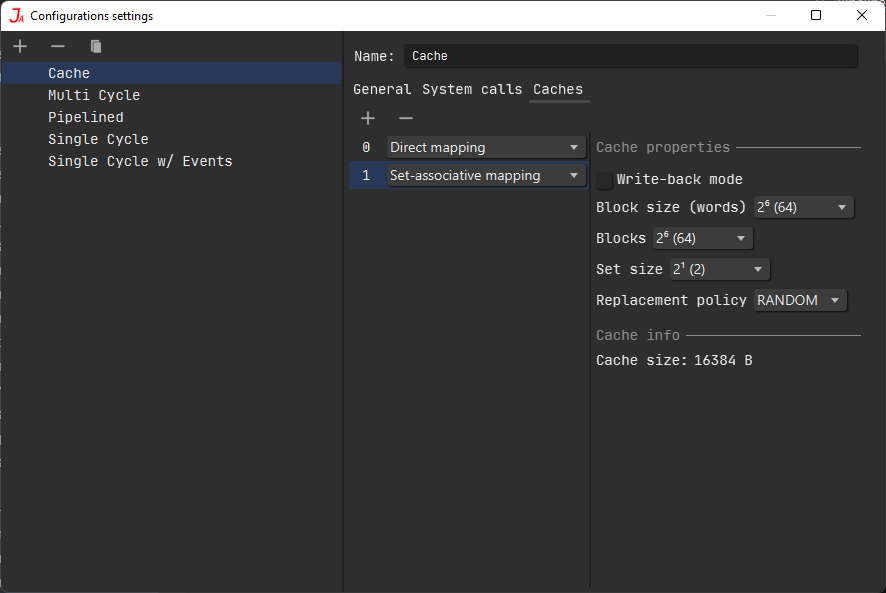
\includegraphics[width=0.8\textwidth]{images/mips/jams-caches}
    \caption{Cachés en las configuraciones del proyecto}
    \label{fig:jams-caches}
\end{figure}

\subsection{Constructores}\label{subsec:constructores}

Para permitir crear nuevos tipos de cachés y memorias,
\textit{JAMS} implementa dos gestores que guardan constructores de cachés
y de memorias.
Estos gestores son $MemoryBuilderManager$ y $CacheBuilderManager$,
los cuales gestionan elementos de tipo
$MemoryBuilder$ y $CacheBuilder$ respectivamente.

\noindent La clase $MemoryBuilder$ es muy sencilla:
contiene un único método que permite crear una nueva memoria.
La clase $CacheBuilder$ es más compleja:
también define propiedades de la caché.
En el gestor estará registrado el constructor con los parámetros por defecto,
mientras que las configuraciones de los proyectos almacenarán copias con los
parámetros deseados.


\section{Simulador}\label{sec:simulador}

Un simulador es una pieza de \textit{software} que imita el comportamiento
de un dispositivo.
\textit{JAMS} implementa diversos simuladores para las diferentes
arquitecturas \textit{MIPS32}.

\subsection{Diferencia entre simulador y emulador}
\label{subsec:diferencia-entre-simulador-y-emulador}

Es importante diferenciar los conceptos de \textbf{simulación}
y \textbf{emulación} a la hora de crear un programa que ejecute
código de arquitecturas externas, como es el caso de \textit{JAMS}.

\noindent Ambos tipos de aplicaciones tienen una finalidad en común:
poder ejecutar código de una arquitectura en otra diferente.
La diferencia se manifiesta en la manera en la que los dos enfoques
se implementan.

\noindent Un emulador tiene como único objetivo el anteriormente
mencionado, y debe cumplirlo de la \textbf{manera más eficiente posible}.
Para ello, recurre a tecnologías como la reconversión del programa
a código nativo.

\noindent Los simuladores toman un enfoque totalmente diferente:
ejecutan el código de la \textbf{manera más fiel posible} a la
arquitectura original, simulando todos los componentes, chips y
buses de datos.
Los simuladores pueden simular la arquitectura en diferentes
niveles: a nivel electrónico, a nivel de puerta lógica, a nivel
de circuito o a nivel de componente.

\noindent En \textit{JAMS} toma mucho más peso en enfoque de la
\textbf{simulación} a nivel de circuito, permitiendo al usuario
conocer el funcionamiento de su aplicación en la arquitectura que desee.
Esto no significa que \textit{JAMS} no optimice la ejecución de código:
todos los componentes están altamente optimizados, pudiendo llegar
la simulación a una velocidad de 40 MHz.

\subsection{Arquitecturas disponibles}\label{subsec:arquitecturas-disponibles}

Actualmente, \textit{JAMS} permite ejecutar el código
en tres arquitecturas \textit{MIPS32} diferentes:
\begin{itemize}
    \item \textbf{Uniciclo}: es la arquitectura más sencilla y
    mejor optimizada.
    Ha sido creada con la velocidad en mente, optando por una
    política de \textbf{cero liberación de memoria}: se crean los mínimos
    objetos posibles, y estos no se liberarán de la memoria hasta que
    la simulación haya terminado.
    Esta política evita que el recolector de basura interfiera en la
    ejecución del simulador, aunmentando su velocidad de ejecución.
    \item \textbf{Multiciclo:} simula una arquitectura
    \textit{MIPS32} multiciclo.
    Es mucho más lenta que la arquitectura uniciclo, ya que requiere
    tener muchos más conceptos en cuenta.
    Las implementaciones de las ejecuciones en esta arquitectura
    están pensadas para ser aprovechadas en arquitecturas más
    complejas, definiendo las lecturas y escrituras de sus
    registros y compartiendo una interfaz transparente para los saltos.
    \item \textbf{Segmentada con varias \textit{ALUs}}: simula
    una arquitectura segmentada o \textit{pipelined} donde coexisten varias
    unidades aritmético-lógicas.
    Esta arquitectura aprovecha mucho código de la arquitectura
    multi-ciclo, y tiende a ser mucho más lenta.
    Los usuarios pueden modificar el número y tipo de las unidades
    aritmético-lógicas, así como el número de ciclos que requiere
    cada una para completar una operación.
\end{itemize}

\subsection{Estructura del simulador}\label{subsec:estructura-del-simulador}

Independientemente de la arquitectura, todas las simulaciones presentan
la misma estructura básica.
Una simulación es un objeto que implementa la interfaz $Simulation$.
Dentro de su clase, se implementa el \textbf{hilo} donde la ejecución
de la simulación toma lugar.
Las simulaciones definen acciones básicas que \textit{JAMS} reflejará en la
aplicación para poder controlar la ejecución: ejecutar, parar, reiniciar
o deshacer un ciclo son algunas de estas acciones.
La interfaz $Simulation$ también define diversos métodos
que permiten acceder a los componentes de la simulación de
manera segura, evitando \textbf{condiciones de carrera}.

\begin{figure}[H]
    \centering
    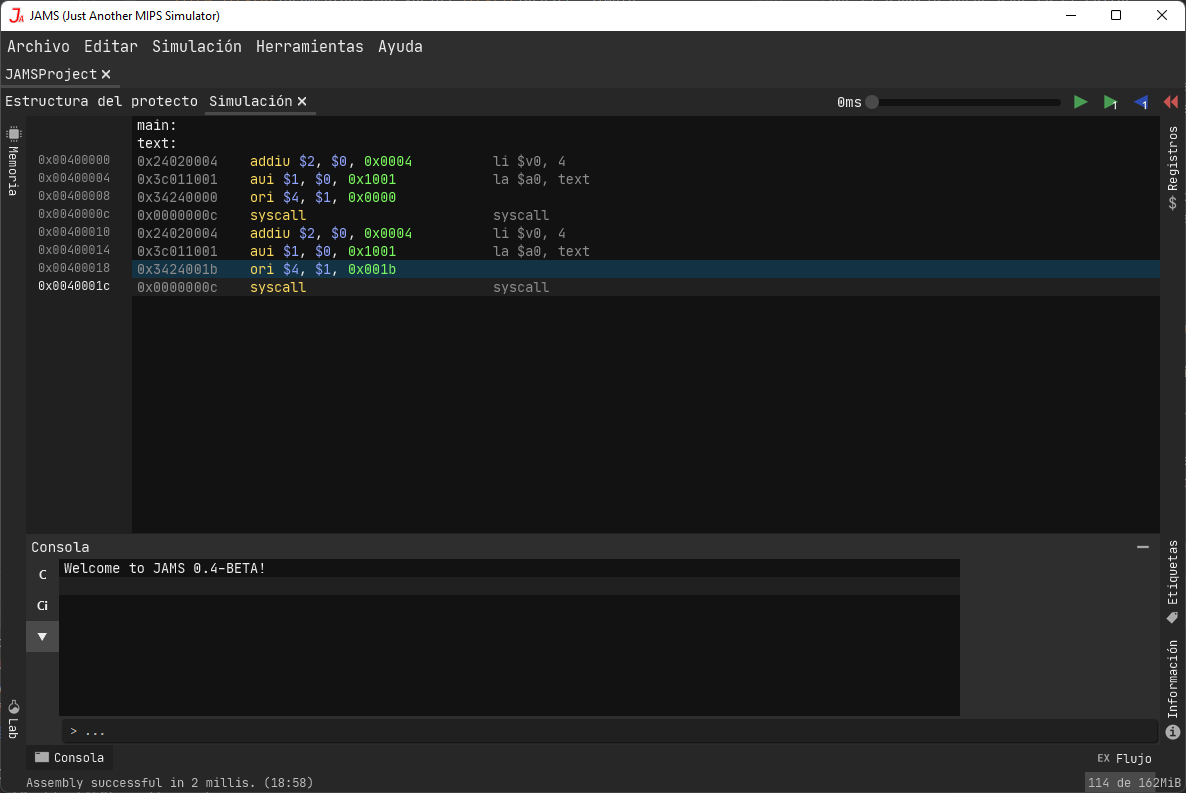
\includegraphics[width=0.8\textwidth]{images/mips/jams-simulation}
    \caption{Interfaz de usuario del simulador}
    \label{fig:jams-simulation}
\end{figure}

\subsection{Interpretación de instrucciones}\label{subsec:interpretación-de-instrucciones}

Una de las operaciones más importantes en un simulador es la búsqueda
de instrucciones y su interpretación.
Este paso es común en todas las arquitecturas: el método $fetch$
incluido en todas las simulaciones \textit{MIPS32} es el encargado
de buscar la instrucción en la memoria, interpretarla y convertirla
en una ejecución adecuada para la arquitectura.

\noindent En las arquitecturas donde una misma instrucción no se puede
ejecutar varias veces al mismo tiempo, este método implementa una
\textbf{caché de ejecuciones}.
Esta caché invalida las instrucciones cuando su representación en
la memoria es modificada, permitiendo al usuario modificar las
instrucciones dentro de la simulación.
Esta caché se llena en el momento en el que la simulación es creada,
realizando un \textit{pre-fetch} de ejecuciones.

\noindent Una vez la simulación consiga la ejecución de la instrucción,
realizará una acción u otra dependiendo de la arquitectura.
Si la arquitectura es una arquitectura uniciclo, el simulador ejecutará
la instrucción invocando el método $execute$ de la ejecución.
Si la arquitectura es una arquitectura multiciclo o segmentada, el simulador
agregará la ejecución en un \textit{pipeline}, e invocará
los métodos $fetch$, $decode$, $execute$, $memory$
o $writeBack$ en el ciclo correspondiente.

\subsection{Registros}\label{subsec:registros}

Un registro es una celda de memoria muy rápida que las instrucciones
utilizan para efectuar sus operaciones.
El procesador \textit{MIPS32} principal implementa 32 registros.

\noindent En \textit{JAMS}, un registro está representado por
una clase que contiene sus diferentes aspectos: identificador, nombres,
si es modificable y su valor por defecto.
La clase también contiene el estado del registro en el estado
actual de una simulación, guardando su valor y
\textbf{una lista con las ejecuciones que están bloqueando el registro}.

\noindent Esta lista es muy importante para determinar el flujo de
las instrucciones en arquitecturas avanzadas, \textbf{permitiendo
detectar y resolver riesgos}.

\subsection{Interrupciones}\label{subsec:interrupciones}

Las interrupciones permiten informar sobre eventos al
simulador.
Cuando una interrupción sucede, el simulador entrará en el
modo \textit{kernel}, saltando automáticamente al controlador
de interrupciones proporcionado por el proyecto.
Si la simulación no tiene implementado ningún controlador de
interrupciones, su ejecución termina de manera abrupta.

\begin{figure}[H]
    \centering
    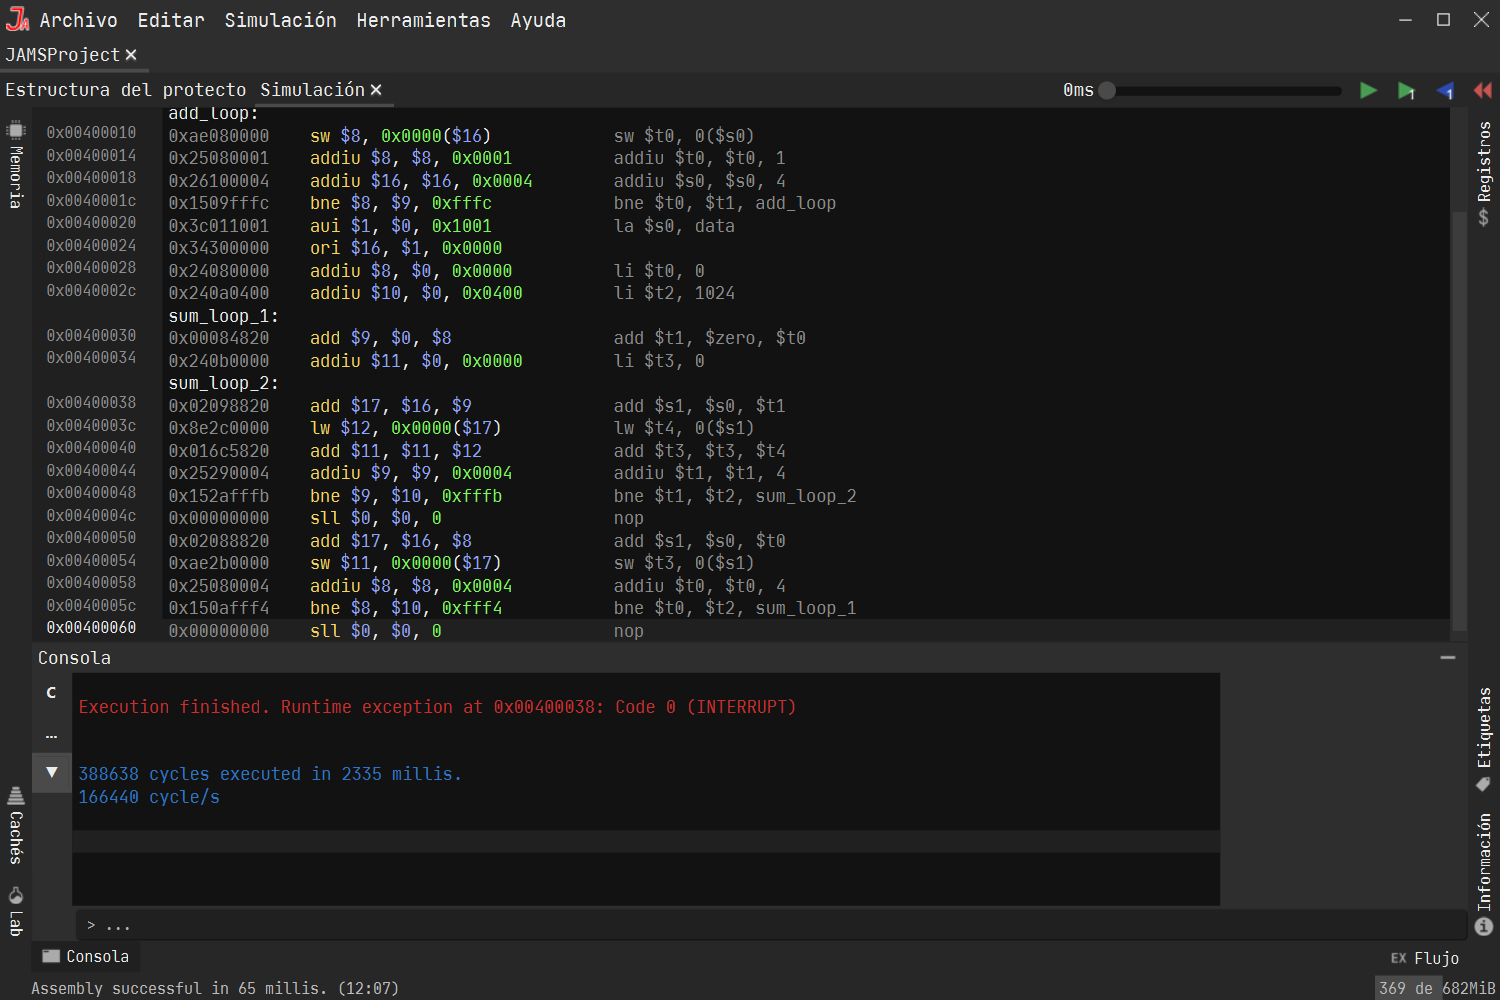
\includegraphics[width=0.8\textwidth]{images/mips/jams-exception}
    \caption{Excepción en una simulación}
    \label{fig:jams-exception}
\end{figure}

\noindent Cuando varias interrupciones ocurren al mismo tiempo,
estas se ejecutan de manera secuencial, teniendo más prioridad
la interrupción \textbf{con mayor nivel}.

\noindent Las interrupciones pueden clasificarse en interrupciones
\textit{software} e interrupciones \textit{hardware}:
\begin{itemize}
    \item \textbf{Interrupciones \textit{software}:} permiten informar
    al programa de errores o excepciones en la simulación.
    Este tipo de interrupciones deben contener una causa que
    el programa puede leer.
    Estas interrupciones son de nivel 1.
    \item \textbf{Interrupciones \textit{hardware}:} permiten informar
    al programa de eventos generados por los diferentes componentes
    conectado al simulador.
    Estas interrupciones están definidas por un nivel entre el
    nivel 2 al 63.
    Este nivel permite calcular la dirección de memoria
    del punto de entrada del controlador de interrupciones.
\end{itemize}

\noindent Los puntos de entrada de los controladores de excepciones
son calculados aplicando el nivel y los parámetros del coprocesador
0 $IntCtl/VS$ (por defecto 1) y $EBase$ (por defecto 0) en la
siguiente expresión:

\[address = EBase + offset \ \& \ 0x3fffffff \ | \ 0x80000000\]

\noindent Donde $offset$ depende del tipo de interrupción:
\begin{itemize}
    \item \textbf{Interrupción \textit{software}:} $0x180$
    \item \textbf{Error de caché:} $0x100$
    \item \textbf{Interrupción \textit{hardware}:} $0x200 + level * VS * 32$
\end{itemize}